\documentclass[12pt, a4paper]{article}

%% Text related
\usepackage[utf8]{inputenc}
\usepackage{indentfirst}
\usepackage[bottom]{footmisc}
\usepackage{verbatim} %Adds comment blocks & code copy-paste
\usepackage[ngerman, num]{isodate} %Proper date format ffs...
    \monthyearsepgerman{}{}
    \daymonthsepgerman{}{}
\usepackage{enumitem}
\usepackage{lipsum} %Because why not?
\usepackage{lscape}

%% Figure related
\usepackage{graphicx}
\usepackage{float} 
\usepackage{subfig}
\usepackage[justification=centering]{caption} %Centers multiline captions

%% Drawing stuff
\usepackage{pgfplots}
\usepackage[american]{circuitikz}

%% Math & Scientific notations
\usepackage{amsmath}
\usepackage{amssymb} %amsmath doesn't have quite common math symbols for some reason
\usepackage[per-mode=repeated-symbol, tight-spacing=true]{siunitx}

%% Table related
\usepackage{multirow}
\usepackage{tabularx}
\usepackage[thinlines]{easytable} %convenient
\usepackage{booktabs} %for different horizontal lines
\usepackage{array} %for table corners not meeting up - doesn't appear to work though

%%
\usepackage{subfiles}

% pgfplots configurations
\graphicspath{ {../img/} }
\pgfplotsset{
    compat=newest,
    standard/.style={
    axis x line=middle,
    axis y line=middle,
    every axis x label/.style={at={(current axis.right of origin)},anchor=west},
    every axis y label/.style={at={(current axis.above origin)},anchor=south}
    }
}

% To place e.g. [ V ] so I don't bother typing it
\newcommand{\unitV}{{\;[\,\SI{}{\volt}\,]}}
\newcommand{\unitmA}{{\;[\,\SI{}{\milli\ampere}\,]}}
\newcommand{\unitA}{{\;[\,\SI{}{\ampere}\,]}}
\newcommand{\unitohm}{{\;[\,\SI{}{\ohm}\,]}}
\newcommand{\unitkohm}{{\;[\,\SI{}{\kilo\ohm}\,]}}

% \title{EED 3009 ENGINEERING DESIGN - II\\FEASIBILITY REPORT}
% \author{Abdurrahman ÜZÜM}
% \date{\today}




\begin{document}

    \begin{titlepage}
        \begin{center}

            \begin{figure}

                \subfloat
                {%
                    
\includegraphics[width=0.3\textwidth]{deulogo.png}
                }
                %
                \hfill
                %
                \subfloat
                {%
                    
\includegraphics[width=0.3\textwidth]{facultylogo.png}
                }

            \end{figure}

            \textbf{T.C.\\}
            \textbf{DOKUZ EYLUL UNIVERSITY\\}
            \textbf{ENGINEERING FACULTY\\}

            \vspace*{1 cm}
            \textbf{ELECTRICAL \& ELECTRONICS ENGINEERING\\}
            \textbf{DEPARTMENT\\}

            \vspace*{1 cm}
            \textbf{EED3009 ENGINEERING DESIGN - II\\}
            \textbf{FEASIBILITY REPORT\\}

            \textbf{RANGE FINDER}

            \vspace*{1 cm}

        
            \begin{table}[H]\centering
                \begin{tabular}{cc}
                    Elif Sezin ÖZYİĞİT \hspace{1cm}  & \hspace{1cm} Abdurrahman ÜZÜM \\
                    2019502098         \hspace{1cm}  & \hspace{1cm} 2019502099       \\             
                \end{tabular}
            \end{table}

            Instructor:\\ Dr.Ogr.Uy.Metehan MAKİNACI\\

            \vspace*{1 cm}
            November, 2022


        \end{center}

    \end{titlepage}



    \pagebreak

    \begin{abstract}
        Early societies measured distance with a variety of primitive tools, from basic paces to measuring rods and marked ropes. Luckily, we’ve come a long way from the days of using belts, thumbs and cubits for measurement. Various methods have been developed over the years in order to increase the measurement accuracy and to be able to measure in various conditions. These devices, which have been developed by human beings step by step over the years and evolved with new technologies, have reached the level where they can measure without the need for physical contact or even light.
    \end{abstract}

    \section{Overview of the Project}

        This project focuses on measuring distances with no contact up to a meter. To realise this project a battery powered, handheld device will be designed. The device will utilise an ultrasonic speaker and microphone. It will send regular periodic ultrasonic bursts from the speaker and listen for the echoes. The necessary circuitry will measure the time between sent ultrasonic bursts and their respective echoes, following the time of flight (ToF) principle. This data will then be processed using necessary information such as the speed of sound on air, as a result of which, the distance data will be obtained. Finally, this distance value will be printed on a two digit display. The device will also employ a laser guide to assist proper alignment of the sensors, and also to provide a feedback to the user. 


        \subsection{Project Inputs}

            \noindent The designed device must
            \begin{itemize}
                \item Measure distances in the range of 0-99\SI{}{\centi\metre}
                \item Have an accuracy of \SI{1}{\centi\metre}
                \item Be battery powered and handheld
                \item Display the measured distance in real time on a two digit display.
                \item Not empoly an MCU or ASIC designed for this particular purpuse.
            \end{itemize}

        
    \pagebreak
    \section{Methodology}
        There are various different possible and applicable approaches for the primary part of the project, the sensors. The first choice is whether to use an optical sensor, or an ultrasonic sensor.

        \subsection{Sensor Types}

            \subsubsection{Optical Sensors}
                Optical sensors themselves have a variety of basis and operation principles, they are classified based on the wawelenght used and principle of operation. In terms of wawelenght most widely used and easily available sensors employ infrared frequencies. 


                \bigskip\noindent
                \textbf{IR - Triangulation Sensors}

                    Commonly these sensors base their measurements on either of the following methods. The IR transmitter, commonly a simple narrow angle LED, continuously emmit light. The beam of light reflects at different angles at different distances, and as a result, falls on different portions of the position-sensitive photodetector (PSD). Knowing the distance between the transmitter and receiver, and calculating the angle of reflection based on where the light struct the receiver, the distance can be calculated using triangulation.

                    \begin{figure}[H]\centering
                        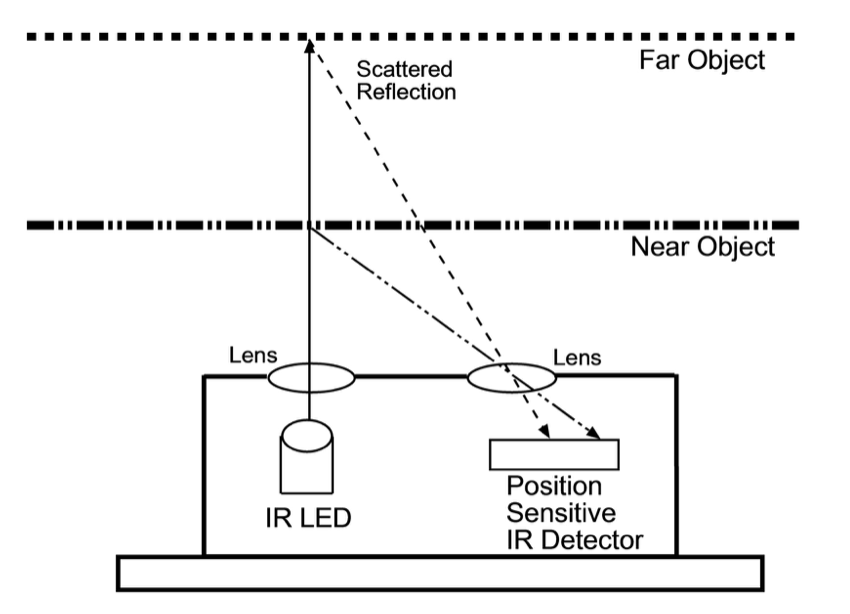
\includegraphics[width=0.5\textwidth]{triangulation}
                        \caption[]{IR Triangulation sensor working principle.}\label{fig:triangulation}
                    \end{figure}
                
                \bigskip\noindent
                \textbf{IR-ToF Sensors}

                    More advanced IR sensors use the time-of-flight (ToF) principle. The emitter sends regular light pulses, a high precision timing circuitry keeps the time it takes for transmitted light to reflect and reach back to the receiver. Knowing the speed of light, distance can be mathematically obtained. These sensors are much less sensitive to the surface material and shape. However, typically optical ToF sensors are much more expensive compared to other types.

                IR sensors can measure the distance of objects with complex surfaces, even if they are affected by environmental conditions and have limited me

                    
            
            \subsubsection{Ultrasonic Sensors}
                Ultrasonic sensors work similarly to ToF IR sensors, only instead of using electromagnetic waves, they utilise sound waves. These sensors also consist of a transmitter (speaker) and a receiver (microphone). Transmitter emmits high frequency ultrasonic sound waves as short bursts, and the receiver listens for echoes. A timing circuitry tracks the time between start of the outgoing burst and the incoming echoed burst. Knowing the speed of sound on air, the distance can easily be calculated.

                Ultrasonic sensors, even with low resolution and slow refresh rate, are really useful because of their long range and low cost.

                \begin{figure}[H]\centering
                    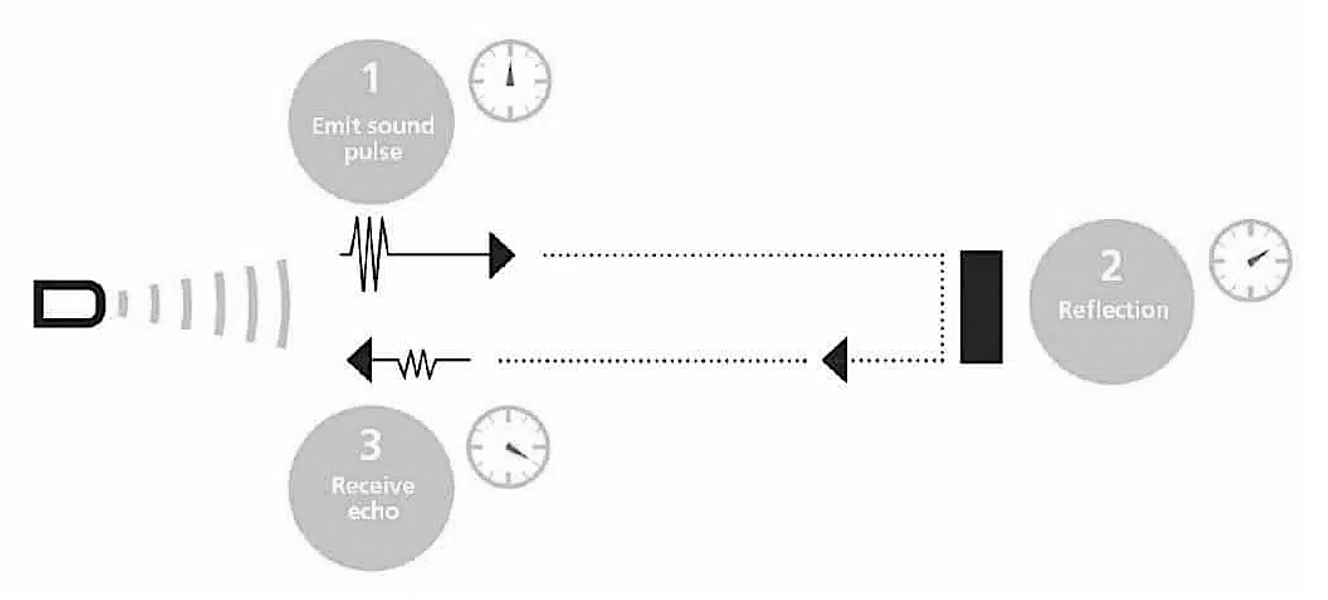
\includegraphics[width=0.8\textwidth]{ultrasonic.png}
                    \caption[]{Ultrasonic ToF sensor working principle.}\label{fig:ultrasonic}
                \end{figure}




        \subsubsection{Comparison}
            In conclusion, IR-Triangulation sensors appear to be the best choice for the distances of interest and the resolution. However, compared to commonly available ultrasonic sensors, they are much more expensive. Due to the reasons mentioned, IR triangular sensors were not considered suitable for the project. Comparing the remaining two options, as tabulated below, clearly shows that the ultrasonic sensor is the better option for the project. Since it was desired to construct a new PCB designed for transducers and to realize the project that way, the idea of designing blocks for an ultrasonic sensor was more attractive and challenging  in personal. The use of ultrasonic sensors makes more sense, both technically and personally.

            \begin{table}[H]\centering
                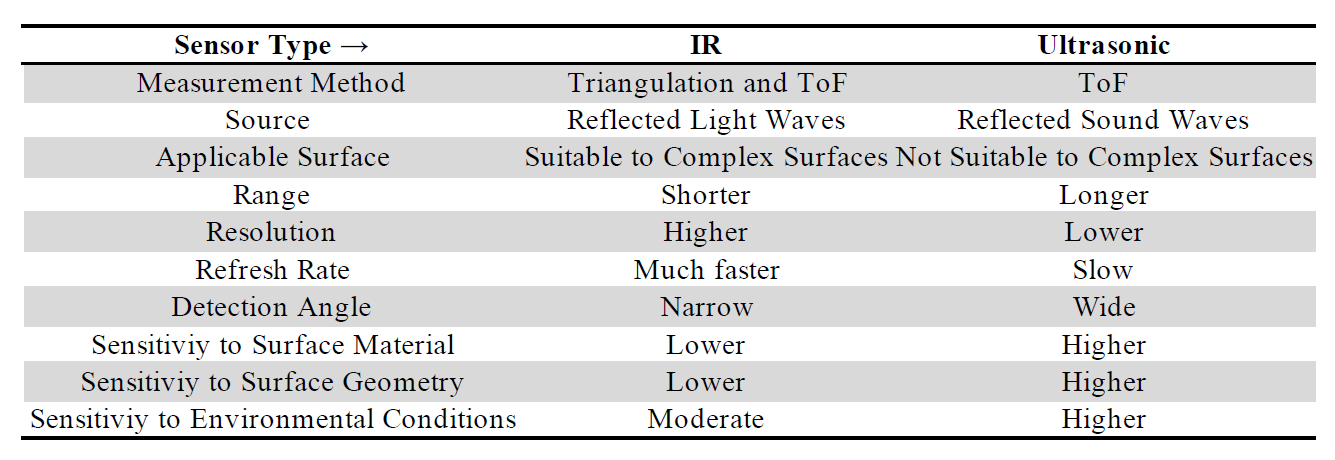
\includegraphics[width=\textwidth]{comparison.png}
                \caption[]{Comparison of two different methods.}\label{tab:comparison}
            \end{table}


    \pagebreak
    \subsection{Design Overview}
        
        \textbf{Giriş girizgah çok boşta kaldı ne yazacğaımı bilemedim}

        Two ultrasonic transducers are needed, one for the transmitter and one for the receiver. The transmitter should be driven periodically with short pulses. The timing between these pulses is critical, such that the following pulse should not be transmitted before the echo of the previous pulse has arrived. This calculation should be made in consideration of the longest distance to be measured. Width of these pulses is also critical, as it should be short enough to ensure that the echo doesn't arrive before the pulse ends. This calculation should be made in considetation of the shortest distance of interest. 

        Assuming that the longest distance to be measured is \SI{100}{\centi\metre}, and speed of sound is \SI{343}{\metre\per\second}, the echo would arrive after:

        \begin{equation}
            \texttt{max }t_f = 2 \times \frac{\SI{1}{\metre}}{\SI{343}{\metre\per\second}} = \SI{5.83}{\milli\second}
        \end{equation}

        \noindent Therefore the time between end of a pulse and start of the other should be around \SI{6}{\milli\second} minimum. 

        \noindent Assuming that the shortest distance to be measured is \SI{1}{\centi\metre}, 

        \begin{equation}
            \texttt{min }t_f = 2 \times \frac{\SI{0.01}{\metre}}{\SI{343}{\metre\per\second}} = \SI{58.3}{\micro\second}
        \end{equation}

        \noindent Therefore the width of the pulse should not exceed about \SI{50}{\micro\second}.


        \bigskip
        Commonly available cheap ultrasonic transducers work at frequencies near \SI{40}{\kilo\hertz}. Therefore the transmitter should send bursts of \SI{40}{\kilo\hertz} sound waves, filling in the previously described pulse. In order to provide a signal with these properties, two generators are needed. One to generate the \SI{40}{\kilo\hertz} signal, and another to generate the pulses. The \SI{40}{\kilo\hertz} signal should then be connected to the transmitter via an analogue switch, which is driven by the pulses.

        \bigskip
        On the receiver side, the received signal will most likely be very low in amplitude, therefore the first stage is to amplify it. This amplification should be made such that the lowest possible echo should not fall short of the limits of the next stage, and the highest possible amplitude echo should not exceed it.
        
        \bigskip
        After the amplification, the \SI{40}{\kilo\hertz} sound burst should be converted into a regular pulse with digital voltage levels. This can be done with a simple envelope detector, and slow rising/falling edges can be converted to digital edges using a logic buffer. 

        \bigskip
        After converting the echo burst into a digital pulse, timing measurements can be done. A counter that is to be started simultaneously with the first edge of the transmitted burst, should then be stopped by the first edge of the echo signal. Output of the counter is proportional to the distance, however, it is necessary to convert it into proper units. For which an arithmetic circuit should follow the counter.

        \bigskip
        After obtaining the meaningful distance data, it then can be transferred to the 7-segment displays. A binary to 7 segment display driver can be employed here for simplicity.

        \pagebreak
        \begin{landscape}\centering
            \vspace*{1.8cm}
            \begin{figure}[H]\centering
                \makebox[\linewidth]
                {
                    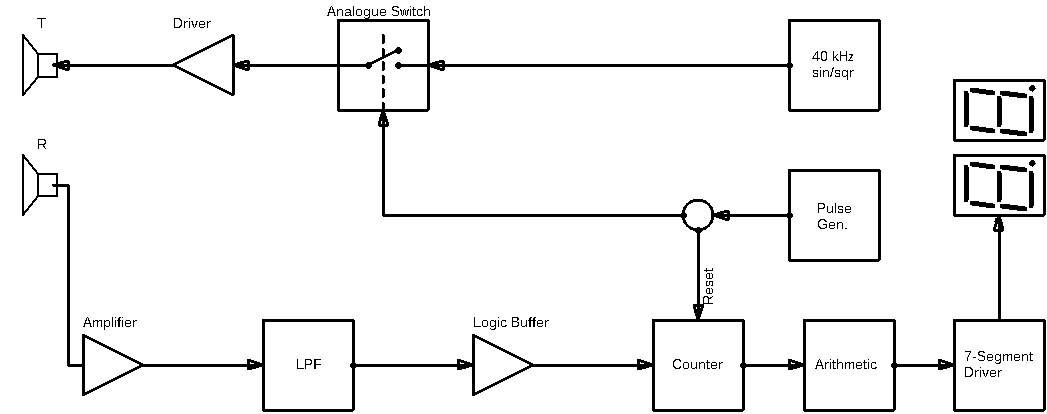
\includegraphics[width=1.2\linewidth]{block2.png}
                }
                \caption{Block Diagram}
            \end{figure}
        \end{landscape}
        \vfill
        \pagebreak


    \section{Technical Feasibility}

        Since HCSR-04 is a cheap and commonly available product it is easier to desolder and salvage the ultrasonic transduces out of it, instead of looking for parts. However, the transducers are not labelled, marked or named, therefore it is not possible to find relevant information about them. Instead, a working HCSR-04 module is put under test and the signal driving the transmitter of the device is observed with an oscilloscope. 

        \noindent On these images, each channel of the scope is connected to one pin of the transmitter, and the purple waveform is the difference between them.

        \begin{figure}[H]\centering
            \includegraphics[width=0.8\textwidth]{experiment1/pulses.png}
            \caption[]{Pulses}\label{fig:pulses}
        \end{figure}

        \noindent As it can be seen, the transmitter is driven with periodic, short pulses. Here, it should be kept in mind that this device uses a microcontroller and tries to be smart, it lenghtens the time between pulses when the distance is longer, and shortens it for shorter distances. Therefore the duration between pulses is not really reliable for this experiement. 

        \begin{figure}[H]\centering
            \includegraphics[width=0.8\textwidth]{experiment1/pulses_close.png}
            \caption[]{Pulses}\label{fig:pulses}
        \end{figure}

        \noindent Here, when zoomed into the short bursts, the \SI{40}{\kilo\hertz} ultrasonic frequency signal can be seen. Note that the transmitter is driven symetrically, but the sensor is powered with positive \SI{5}{\volt}, therefore the module has decided to drive the transmitter with alternating \SI{5}{\volt} square pulses on either pin and obtaining a symmetrical \SI{10}{\volt} square wave. 

        \begin{figure}[H]\centering
            \includegraphics[width=0.8\textwidth]{experiment1/pulses_duration.png}
            \caption[]{Pulses}\label{fig:pulses}
        \end{figure}

        \begin{figure}[H]\centering
            \includegraphics[width=0.8\textwidth]{experiment1/ultrasonic_freq_amplt.png}
            \caption[]{Pulses}\label{fig:pulses}
        \end{figure}



        \pagebreak
        In order to test the behaviours of transducers, they are desoldered from the module and soldered back on an empty prototyping board. It is necessary to measure what the received signal amplitude will be in order to design a proper amplifier.

        $\SI{10}{\volt}_{\texttt{pp}}$ \SI{40}{\kilo\hertz} sinusoidal signal is applied to the transmitter directly from a function generator and output of the receiver is measured using the oscilloscope. Amplitude of the received signal is observed at various distances. 

        It is observed that the received signal amplitude drops below \SI{100}{\milli\volt} for very large distances (not shown on the pictures). At about 40-50 \SI{}{\centi\metre}, the signal amplitude is about \SI{200}{\milli\volt}, and for very close distances at about 5-10 \SI{}{\centi\metre}, amplitude reaches \SI{800}{\milli\volt}. 

        \begin{figure}[H]\centering
            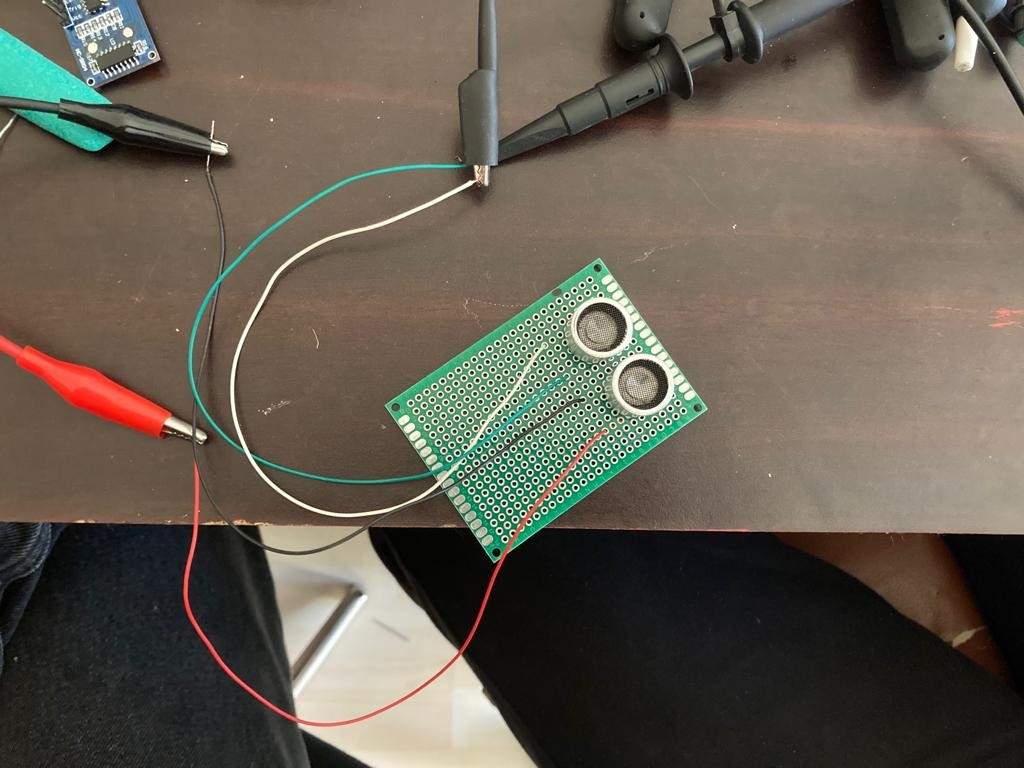
\includegraphics[width=\textwidth]{experiment2/setup.jpg}
            \caption[]{Experiment setup}\label{fig:setup}
        \end{figure}

        \begin{figure}[H]\centering
            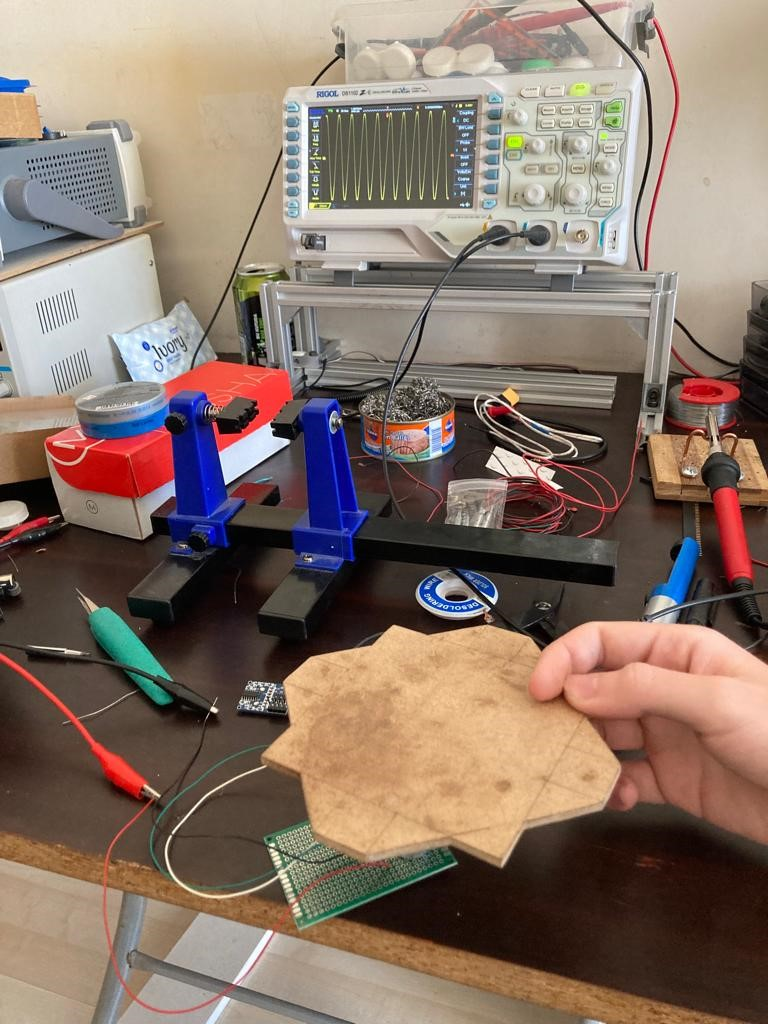
\includegraphics[width=0.5\textwidth]{experiment2/near.jpg}
            \caption[]{}\label{fig:near}
        \end{figure}

        \begin{figure}[H]\centering
            \includegraphics[width=\textwidth]{experiment2/near_scope.png}
            \caption[]{}\label{fig:ner_scope}
        \end{figure}


        \begin{figure}[H]\centering
            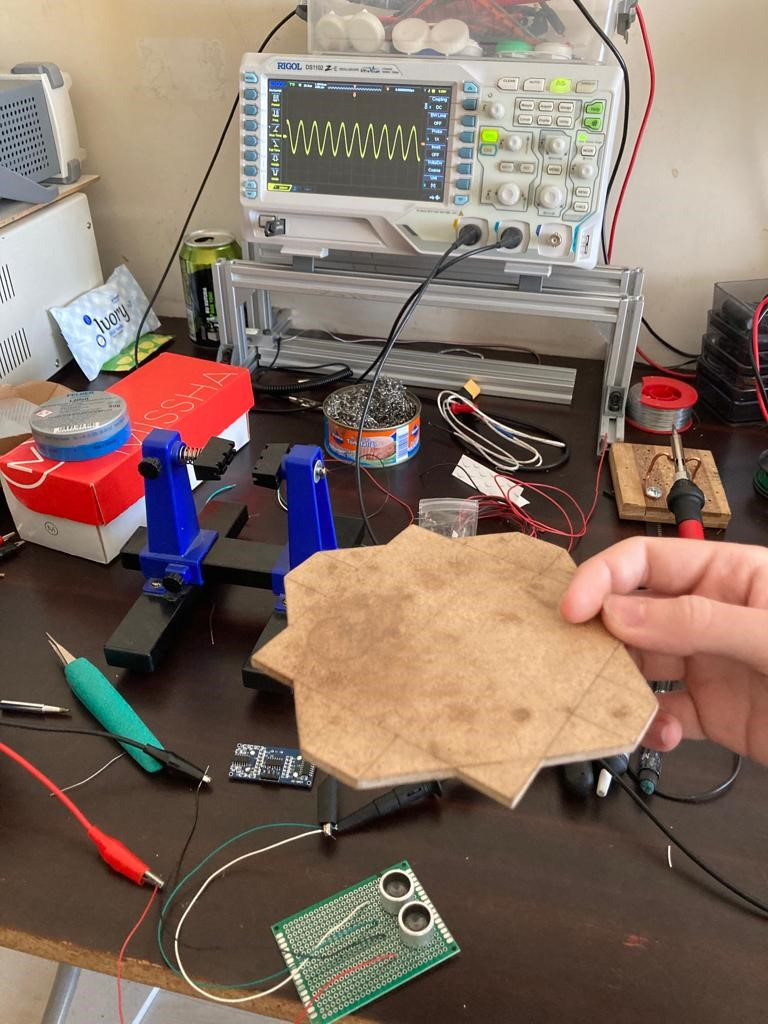
\includegraphics[width=0.5\textwidth]{experiment2/medium.jpg}
            \caption[]{}\label{fig:medium}
        \end{figure}

        \begin{figure}[H]\centering
            \includegraphics[width=\textwidth]{experiment2/medium_scope.png}
            \caption[]{}\label{fig:medium_scope}
        \end{figure}


        \begin{figure}[H]\centering
            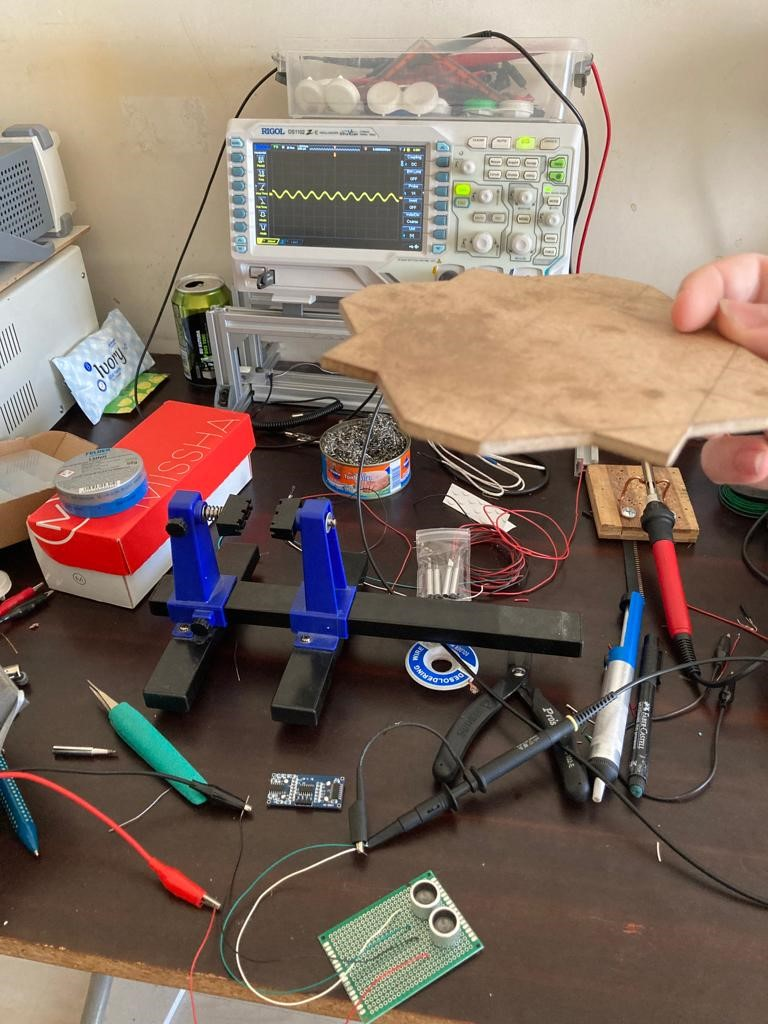
\includegraphics[width=0.5\textwidth]{experiment2/far.jpg}
            \caption[]{}\label{fig:far}
        \end{figure}

        \begin{figure}[H]\centering
            \includegraphics[width=\textwidth]{experiment2/far_scope.png}
            \caption[]{}\label{fig:far_scope}
        \end{figure}


        





    
    \section{Cost Analysis}

        The following table shows the components to be used based on first draft design of the project. All of these componets and given prices are subject to change as the design is going through revisions and further considerations.
        
        \begin{table}[H]\centering
            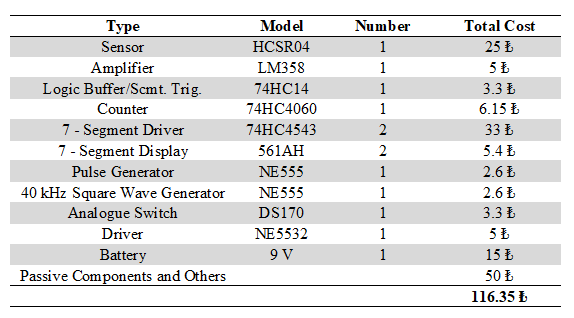
\includegraphics[width=\textwidth]{cost.png}
            \caption[]{Cost Analysis Table}\label{tab:cost}
        \end{table}

    \section{Risk Feasibility}

    \pagebreak
    \section{Gannt Chart}

        \begin{figure}[H]\centering
            \makebox[\linewidth]
                {
                    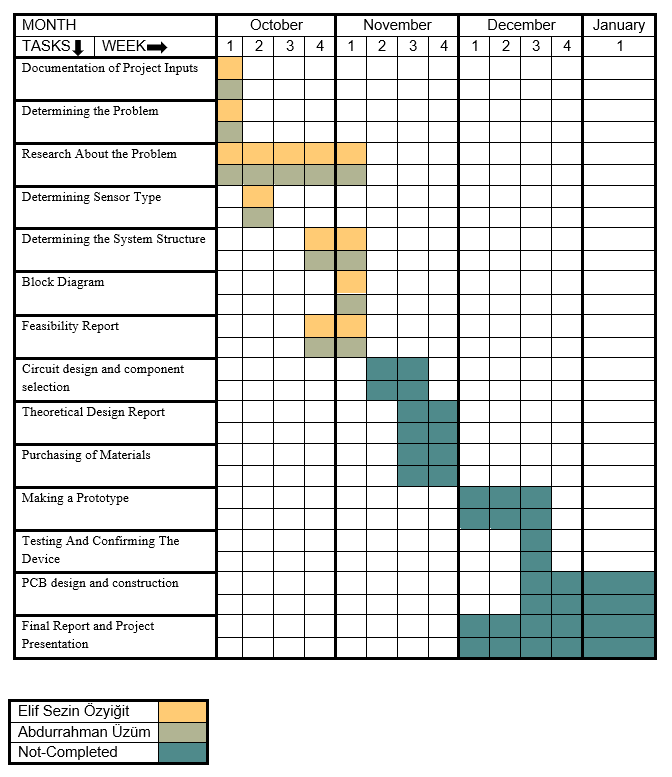
\includegraphics[width=1.2\linewidth]{ganntchart.png}
                }
                \caption{Gannt Chart}
        \end{figure}



            





\end{document}